%% LyX 2.3.2 created this file.  For more info, see http://www.lyx.org/.
%% Do not edit unless you really know what you are doing.
\documentclass[english]{llncs}
\usepackage[T1]{fontenc}
\usepackage[latin9]{inputenc}
\usepackage{amssymb}
\usepackage{stmaryrd}
\usepackage{graphicx}
\usepackage{setspace}
\usepackage[authoryear]{natbib}
\onehalfspacing

\makeatletter

%%%%%%%%%%%%%%%%%%%%%%%%%%%%%% LyX specific LaTeX commands.
%% Because html converters don't know tabularnewline
\providecommand{\tabularnewline}{\\}

\makeatother

\usepackage{babel}
\begin{document}
\title{Dataset mention extraction in scientific articles using a BiLSTM-CRF
model}
\author{Tong Zeng$^{1,2}$ and Daniel Acuna$^{1}$\thanks{Corresponding author: deacuna@syr.edu}}
\institute{$^{1}$School of Information Studies, Syracuse University, Syracuse,
USA\\
$^{2}$School of Information Management, Nanjing University, Nanjing,
China}
\maketitle
\begin{abstract}
Datasets are critical for scientific research, playing a role in replication,
reproducibility, and efficiency. Researchers have recently shown that
datasets are becoming more important for science to function properly,
even serving as artifacts of study themselves. However, citing datasets
is not a common or standard practice in spite of recent efforts by
data repositories and funding agencies. This greatly affects our ability
to track their usage and importance. A potential solution to this
problem is to automatically extract dataset mentions from scientific
articles. In this work, we propose to achieve such extraction by using
a neural network based on a BiLSTM-CRF architecture. Our method achieves
$F_{1}=0.885$ in social science articles released as part of the
Rich Context Dataset. We discuss future improvements to the model
and applications beyond social sciences.
\end{abstract}


\section{Introduction}

Science is fundamentally an incremental discipline that depends on
previous scientist's work. Datasets form an integral part of this
process and therefore should be shared and cited as any other scientific
output. This ideal is far from reality: the credit that datasets currently
receive does not correspond to their actual usage. One of the issues
is that there is no standard for citing datasets, and even if they
are cited, they are not properly tracked by major scientific indices.
Interestingly, while datasets are still used and mentioned in articles,
we lack methods to extract such mentions and properly reconstruct
dataset citations. The Rich Context Competition challenge aims at
closing this gap by inviting scientists to produce automated dataset
mention and linkage detection algorithms. In this article, we detail
our proposal to solve the dataset mention step. Our approach attempts
to provide a first approximation to better give credit and keep track
of datasets and their usage.

The problem of dataset extraction has been explored before. \citet{ghavimiIdentifyingImprovingDataset2016}
and \citet{ghavimiSemiautomaticApproachDetecting2017} use a relatively
simple tf-idf representation with cosine similarity for matching dataset
identification in social science articles. Their method consists of
four major steps: preparing a curated dictionary of typical mention
phrases, detecting dataset references, and ranking matching datasets
based on cosine similarity of tf-idf representations. This approach
achieved a relatively high performance, with $F_{1}=0.84$ for mention
detection and $F_{1}=0.83$, for matching. \citet{singhalDataExtractMining2013}
proposed a method using normalized Google distance to screen whether
a term is in a dataset. However, this method relies on external services
and is not computational efficient. They achieve a good $F_{1}=0.85$
using Google search and $F_{1}=0.75$ using Bing. A somewhat similar
project was proposed by \citet{luDatasetSearchEngine2012}. They built
a dataset search engine by solving the two challenges: identification
of the dataset and association to a URL. They build a dataset of 1000
documents with their URLs, containing 8922 words or abbreviations
representing datasets. They also build a web-based interface. This
shows the importance of dataset mention extraction and how several
groups have tried to tackle the problem.

In this article, we describe a method for extracting dataset mentions
based on a deep recurrent neural network. In particular, we used a
Bidirectional Long short-term Memory (BiLSTM) sequence to sequence
model paired with a Conditional Random Field (CRF) inference mechanism.
We tested our model on a novel dataset produced for the Rich Context
Competition challenge. We achieve a relatively good performance of
$F_{1}=0.885$. We discuss the limitations of our model.

\section{The dataset}

The Rich Context Dataset challenge was proposed by the New York University's
Coleridge Initiative \citep{richtextcompetition}. The challenge comprised
several phases, and participants moved through the phases depending
on their performance. We only analyze data of the first phase. This
phase contained a list of datasets and a labeled corpus of around
5K publications. Each publication was labeled indicating whether a
dataset was mentioned within it and which part of the text mentioned
it. The challenge used the accuracy for measuring the performance
of the competitors and also the quality of the code, documentation,
and efficiency.

We adopt the CoNLL 2003 format \citep{tjong2003introduction} to annotate
whether a token is a part of dataset mention. Concretely, B-DS denotes
a token that is the first token of a dataset mention, I-DS denotes
a token that is inside of dataset mention, and O denotes a token that
is not a part of dataset mention. We then put each token and its corresponding
labels in one line and use a empty line as a separator between sentences.
Sentences were randomly split by 70\%, 15\%, 15\% for training set,
validation set and testing set, respectively.

\section{The Proposed Method}

\subsection{Overall view of the architecture}

In this section, we propose a model for detecting mentions based on
a BiLSTM-CRF architecture. At a high level, the model uses a sequence-to-sequence
recurrent neural network that produces the probability of whether
a token belongs to a dataset mention. The CRF layer takes those probabilities
and estimates the most likely sequence based on constrains between
label transitions (e.g., mention--to--no-mention--to-mention has
low probability). While this is a standard architecture for modeling
sequence labeling, the application to our particular dataset and problem
is new.

We now describe in more detail the choices of word representation,
hyper-parameters, and training parameters. A schematic view of the
model is in Fig \ref{fig:NetworkArchitecture} and the components
are as follows:
\begin{enumerate}
\item Character embedding layer: treat a token as a sequence of characters
and encode the characters by using a bidirectional LSTM to get a vector
representation.
\item Word embedding layer: mapping each token into fixed sized vector representation
by using a pre-trained word vector.
\item One BiLSTM layer: make use of Bidirectional LSTM network to capture
the high level representation of the whole token sequence input.
\item Dense layer: project the output of the previous layer to a low dimensional
vector representation of the the distribution of labels.
\item CRF layer: find the most likely sequence of labels.
\end{enumerate}
\begin{figure}
\begin{centering}
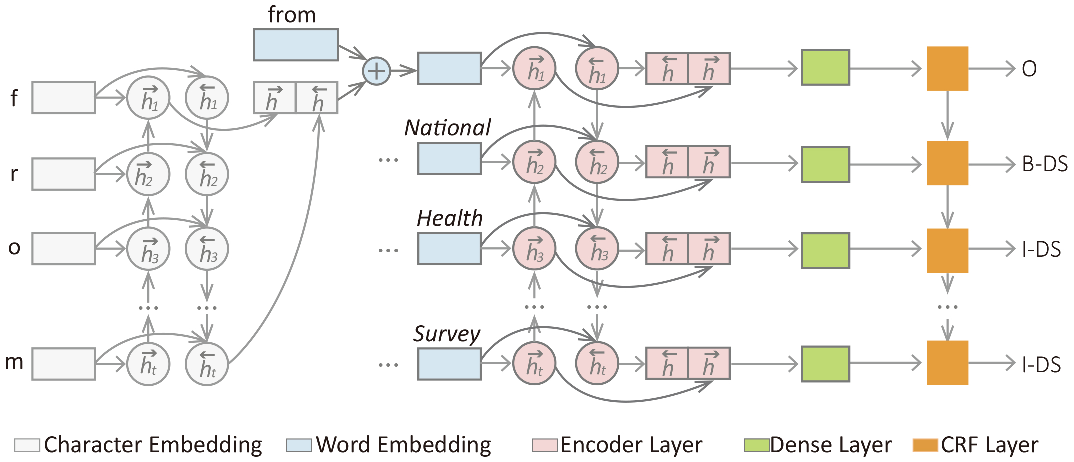
\includegraphics[width=0.8\textwidth]{img/bilistm_crf_network_structure_pic}
\par\end{centering}
\caption{\label{fig:NetworkArchitecture}Network Architecture of BiLSTM-CRF
network}
\end{figure}


\subsection{Character Embedding}

Similar to the bag of words assumption, we can consider a token is
composed by a bag of characters. In this layer, we convert each token
to a sequence of characters, then feed the sequence into a bidirectional
LSTM network to get a fixed length representation of the token. After
learning the bidirectional LSTM network, we can solve the out-of-vocabulary
problem for pre-trained word embeddings.

\subsection{Word Embedding}

The embedding is the first layer of our network and it is responsible
for mapping the word from string into vectors of numbers as the input
for other layers on top. For a given sentence $S$, we first convert
it into a sequence consisting of $n$ tokens, $S=\{c_{1},c_{2},\cdots,c_{n},\}$
. For each token $c_{i}$we lookup the embedding vector $x_{i}$ from
a word embedding matrix $M^{tkn}\in\mathbb{R}^{d|V|}$, where the
$d$ is the dimension of the embedding vector and the $V$ is the
Vocabulary of the tokens. In this paper, the matrix $M^{tkn}$ is
initialized by pre-trained GloVe vectors \citep{pennington2014glove},
but will be updated by learning from our corpus.

\subsection{LSTM}

Recurrent neural network (RNN) is a powerful tool to capture features
from sequential data, such as temporal series, and text. RNN could
capture long-distance dependency in theory but it suffers from the
gradient exploding/vanishing problems \citep{pascanu2013difficulty}.
The Long short-term memory (LSTM) architecture was proposed by \citet{hochreiter1997long}
and it is a variant of RNN which copes with the gradient problem.
LSTM introduces several gates to control the proportion of information
to forget from previous time steps and to pass to the next time step.
Formally, LSTM could be described by the following equations:

\begin{equation}
i_{t}=\sigma(W_{i}x_{t}+W_{i}h_{t-1}+b_{i})
\end{equation}
\begin{equation}
f_{t}=\sigma(W_{f}x_{t}+W_{f}h_{t-1}+b_{f})
\end{equation}
\begin{equation}
g_{t}=tanh(W_{g}x_{t}+W_{g}h_{t-1}+b_{g})
\end{equation}
\begin{equation}
o_{t}=\sigma(W_{o}x_{t}+W_{o}h_{t-1}+b_{o})
\end{equation}
\begin{equation}
c_{t}=f_{t}\bigotimes c_{t-1}+i_{t}\bigotimes g_{t}
\end{equation}
\begin{equation}
h_{t}=o_{t}\bigotimes tanh(c_{t})
\end{equation}
where the $\sigma$ is the sigmoid function, $\bigotimes$ denotes
the dot product, $b$ is the bias, $W$ is the parameters, $x_{t}$
is the input at time $t$, $c_{t}$ is the LSTM cell state at time
$t$ and $h_{t}$ is hidden state at time $t$. The $i_{t}$, $f_{t}$,
$o_{t}$ and $g_{t}$ are named as input, forget, output and cell
gates respectively, they control the information to keep in its state
and pass to next step.

LSTM gets information from the previous steps, which is left context
in our task. However, it is important to consider the information
in the right context. A solution of this information need is bidirectional
LSTM \citep{graves2013speech}. The idea of Bi-LSTM is to use LSTM
layers and feed the forward and backward flows separately, and then
concatenate the hidden states of the two LSTM to modeling both the
left and right contexts

\begin{equation}
h_{t}=[\overrightarrow{h_{t}}\varoplus\overleftarrow{h_{t}}]
\end{equation}

Finally, the outcomes of the states are taken by a Conditional Random
Field (CRF) layer that takes into account the transition nature of
the beginning, intermediate, and ends of mentions. For a reference
of CRF, refer to \citep{lafferty2001conditional}

\section{Results}

In this work, we wanted to propose a model for the Rich Context Competition
challenge. We propose a relatively standard architecture based on
a BiLSTM-CRF recurrent neural network. We now describe the results
of this network on the dataset provided by the competition.

For all of our results, we use $F_{1}$ as the measure of choice.
This measure is the harmonic average of the precision and recall and
it is the standard measure used in sequence labeling tasks. This metric
varies from 0 to 1, and the unit is the highest possible value. Our
method achieved a relatively high $F_{1}$ of 0.885 for detecting
mentions, in line with previous studies.
\begin{table}
\caption{\label{tab:Performance-of-proposed}Performance of proposed network}

\centering{}%
\begin{tabular}{cccccc}
\hline 
Models & GloVe size & Dropout rate & Precision & Recall & $F_{1}$\tabularnewline
\hline 
m1 & 50 & 0.0 & 0.884 & 0.873 & 0.878\tabularnewline
m2 & 50 & 0.5 & 0.877 & 0.888 & 0.882\tabularnewline
m3 & 100 & 0.0 & 0.882 & 0.871  & 0.876\tabularnewline
m4 & 100 & 0.5 & 0.885 & 0.885 & \textbf{0.885}\tabularnewline
m5 & 200 & 0.0 & 0.882 & 0.884  & 0.883\tabularnewline
m6 & 200 & 0.5 & 0.885 & 0.880 & 0.882\tabularnewline
m7 & 300 & 0.0 & 0.868 & 0.886 & 0.877\tabularnewline
m8 & 300 & 0.5 & 0.876 & 0.878 & 0.877\tabularnewline
\hline 
\end{tabular}
\end{table}

We train models using the training data, monitor the performance using
the validation data (we stop training if the performance doesn't improve
for the last 10 epochs). We are using the Adam optimizer with learning
rate of 0.001 and batch size equal to 64. The hidden size of LSTM
for character and word embedding is 80 and 300, respectively. For
the regularization methods to avoid over-fitting, we use L2 regularization
with alpha set to 0.01, we also use dropout rate equal to 0.5. We
trained 8 models with a combination of different GloVe vector size
(50, 100, 300 and 300) and dropout rate (0.0, 0.5). The performances
are reported on the test dataset in Table \ref{tab:Performance-of-proposed}.
The best model is trained by word vector size 100 and dropout rate
0.5 with $F_{1}$ score 0.885.

We also found some limitations to the dataset. Firstly, we found that
mentions are nested (e.g. HRS, RAND HRS, RAND HRS DATA are linked
to the same dataset). The second issue most of the mentions have ambiguous
relationships to datasets. In particular, only 17,267 (16.99\%) mentions
are linked to one dataset, 15,292 (15.04\%) mentions are listed to
two datasets, and 12,624 (12.42\%) are linked to three datasets. If
these difficulties are not overcome, then the predictions from the
linkage process will be noisy and therefore impossible to tell apart.

\section{Conclusion}

In this work, we report a high accuracy model for the problem of detecting
dataset mentions. Because our method is based on a standard BiLSTM-CRF
architecture, we expect that updating our model with recent developments
in neural networks would only benefit our results. We also provide
some evidence of how difficult we believe the linkage step of the
challenge could be if the dataset noise are not lowered. 

One of the shortcomings of our approach is that the architecture is
lacking some modern features of RNN networks. In particular, recent
work has shown that attention mechanisms are important especially
when the task requires spatially distant information, such as this
one. These benefits could also translate to better linkage. We are
exploring new architectures using self-attention and multiple-head
attention. We hope to explore these approaches in the near future.

Our proposal, however, is surprisingly effective. Because we have
barely modified a general RNN architecture, we expect that our results
will generalize relatively well either to the second phase of the
challenge or even to other disciplines. We would emphasize, however,
that the quality of the dataset has a great deal of room for improvement.
Given how important this task is for the whole of science, we should
try to strive to improve the quality of these datasets so that techniques
like this one can be more broadly applied. The importance of dataset
mention and linkage therefore could be fully appreciated by the community. 

\section*{Acknowledgements}

Tong Zeng was funded by the China Scholarship Council \#201706190067.
Daniel E. Acuna was funded by the National Science Foundation awards
\#1646763 and \#1800956.

\bibliographystyle{apalike}
\bibliography{rcc-06}

\end{document}
